\section{Reševanje enačb}
\label{pogl:enacbe}


\textcolor{red}{popravi da so captioni slik, ki so v več kot eni vrstici, poravbnani na sredini}

Zapustimo deloma področje geometrije in si poglejmo, kako lahko s prepogibanjem papirja rešujemo enačbe z racionalnimi koeficienti.

Spomnimo se še, da smo origami-konstruktibilna števila definirali kot vsa števila, ki jih lahko s prepogibanjem konstruiramo preko na začetku dane abscine osi, izhodišča $(0,0)$ in točke $(1,0)$ in da lahko kar predpostavimo, da imamo dan celoten koordinatni sistem z abscisno in ordinatno osjo, izhodiščem ter enoto $1$ na obeh oseh (definicija~\ref{def:origami_konstruktibilnost}). V tej ravnini bomo konstruirali rešitve naših enačb, da pa bo pregibov čim manj in s tem preglednost večja, lahko pomožne točke in premice narišemo kar s svinčnikom (ker bi jih tako ali tako znali konstruirati s pregibi).

Začnimo z najbolj osnovno, t.\ j.\ linearno enačbo. Enačba $ax + b = 0$, kjer $a, b \in \Q$ in $a \neq 0$ ima rešitev $x = -b/a$, ki je racionalno število in po izreku~\ref{izr:origami_konstruktibilnost} origami-konstruktibilno. Če bi želeli rešitev konstruirati z origamijem in geometrijsko, v ravnini prepognemo premico $y = ax + b$ (napravimo pregib npr.\ skozi točki (0, b) in (1, a+b)) in njeno presečišče z abscisno osjo nam da iskano rešitev.

Uporaba origamija je za reševanje linearne enačbe očitno manj praktična kot računanje rešitve. Bolj zanimivo je reševanje kvadratne in kubične enačbe. Ker za njune rešitve obstajata splošni formuli, bi jih lahko najprej izračunali in nato preko operacij seštevanja, odštevanja, množenja, deljenja in korenjenja konstruirali s prepogibanjem, vendar je to časovno preveč potratno. Pogledali si bomo, kako se z origamijem lahko temu izognemo in rešitev konstruiramo bolj direktno.

Ključno vlogo bosta v nadaljevanju odigrali origami operaciji~\ref{op:O6} in~\ref{op:O7}. Prva nam hkrati s konstrukcijo tangente na parabolo določi tudi točko na paraboli, skozi katero je pregib tangenten na stožnico, to pa je ekvivalentno reševanju kvadratne enačbe. Druga pa s konstrukcijo skupne tangente na dve paraboli omogoča reševanje kubične enačbe. Alperin v~\cite[str.\ 129]{alperin2000} pokaže, kako izpeljati kubično enačbo za koeficient skupne tangente na dani paraboli. Število rešitev kubične enačbe je torej enako številu skupnih tangent, kar pomeni, da imata paraboli v evklidski ravnini največ tri skupne tangente.

V teoriji bi nam prepogibanje papirja pomagalo tudi pri reševanju kvartičnih enačb, saj zanje še obstaja splošna formula in tudi vemo, da lahko enačbo četrte stopnje prevedemo na enačbe nižje stopnje (gl.\ \cite{wikiquartic}, \cite{quartics2012}). Praktično pa je to težje izvedljivo, saj bi postopek reševanja zahteval veliko več pregibov kot pri reševanju ene kubične ali kvadratne enačbe, pa tudi vmesne rezutate bi morali računati. (\textcolor{red}{Poglej članek~\cite{edwards2001} (naložen), ker mogoče je pa tle dejansko urjdi postopek za reševanje enačb 4.\ stopnje})

Za enačbe pete in višjih stopenj pa splošna formula za rešitve ne obstaja več (\emph{Abel-Ruffinijev} izrek, gl.\ \cite{mrinal2019}). Kljub temu se da z origamijem še vedno konstruirati rešitve nekaterih enačb višjih stopenj, vendar ne obstaja postopek z enkratnimi prepogibi -- potrebno se je poslužiti dvojnih (\emph{two fold}) ali večkratnih (\emph{multi-fold}) prepogibov (gl.\ poglavje~\ref{pogl:multifold}).

\subsection{Kvadratna enačba}
\label{podpogl:kvadratna_enacba}

Rešujemo enačbo oblike
$$ a x^2 + b x + c = 0, $$
kjer so $a, b, c \in \Q$ in velja $a \neq 0$.  Njeni splošni rešitvi sta
$$ x_{1,2} = \frac{-b \pm \sqrt{b^2 - 4ac}}{2a},$$ vendar so konstrukcije vseh teh števil časovno potratno, zato iščemo hitrejši način reševanja.

Postopek, ki si ga bomo pogledali v nadaljevanju, predpostavlja $a = 1$. Ker je vodilni koeficient neničeln, lahko z njim enačbo delimo in pri tem še vedno dobimo racionalne koeficiente, zato lahko predpostavko brez škode za splošnost sprejmemo. Nova oblika enačbe je tako
\begin{equation}
    \label{eq:spl_kv_en}
    x^2 + bx + c = 0.
\end{equation}
Predpostavimo, da ima enačba dve različni realni rešitvi oz.\ da je diskriminanta enačbe pozitivna, t.\ j.\ $D = b^2 - 4c > 0$. Če realnih ničel ni, o origami konstrukciji rešitev namreč nima smisla razpravljati. Če je rešitev ena, je podana kot $x = -b/2$, kar je origami-konstruktibilno število in se ga lahko takoj konstruira.

Enačba~\ref{eq:spl_kv_en} nam poda pokončno parabolo $y = x^2 + bx + c$ z vodoravno premico vodnico in dvema ničlama, ki sta rešitvi naše enačbe. Iščemo absciso presečišča parabole z abscisno osjo.

Zopet se bomo poslužili dosedanjega znanja o operaciji~\ref{op:O6}. Ta nam s pregibom skozi dano točko $B$, ki točko $A$ položi na premico $a$, konstruira tangento na parabolo z goriščem v točki $A$ in premico vodnico $a$.

Naša parabola je z enačbo seveda natančno določena. Ideja iskane konstrukcije rešitev enačbe je določiti tako točko $B$ (najlažje kar na osi parabole), da bi nam izvedba operacije~\ref{op:O6} podala tangento na parabolo ravno v njeni ničli. Želeni pregib mora potekati skozi točko $B$ in gorišče $A$ položiti na tisto točko $A'$ na premici vodnici $a$, ki ima enako absciso kot ničla parabole. (gl.\ sliko~\ref{fig:tockaB_in_O6}). Taka točka $B$ je z osjo parabole in katerokoli izmed ničlama (zaradi simetrije) natanko določena.

\begin{figure}[h]
    \centering
    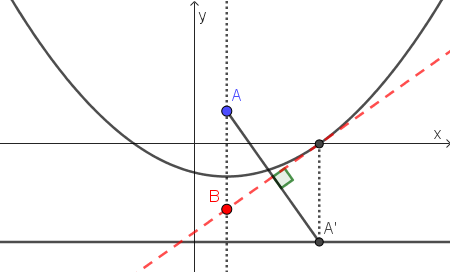
\includegraphics[width=0.5\textwidth]{images/kvadratna_enacba/tockaB_in_O6.png}
    \caption[Iskanje točke $B$]{Operacijo~\ref{op:O6} skozi iskano točko $B$ poda rešitev kvadratne enačbe.}
    \label{fig:tockaB_in_O6}
\end{figure}

Edina nevarnost, da ta konstrukcija ne bo delovala, je možnost, da točka $B$ kdaj ne bo origami-konstruktibilna točka. Zato sedaj izračunajmo njene koordinate in se prepričajmo, da se to nikoli ne bo zgodilo.

Najprej iz dane enačbe parabole določimo njeno gorišče $A$ in premico vodnico $a$. Spomnimo se, da iz enačbe parabole oblike
$$ (x - x_0)^2 = 2p(y - y_0) $$
takoj razberemo koordinati gorišča $(x_0, y_0)$ in enačbo premice vodnice $y = y_0 - p$. V našem primeru enačbo $y = x^2 + bx + c$ preoblikujemo v
$$ \left(x-\left(-\frac{b}{2}\right)\right)^2 = 2 \cdot \frac{1}{2} \left(y - \left(c - \frac{b^2}{4}\right)\right). $$
S tem sta gorišče $A$ in premica vodnica $a$ določena:
$$ A\left(-\frac{b}{2}, c - \frac{b^2 - 1}{4}\right) \text{ in } a: y = c - \frac{b^2 + 1}{4}. $$

Naj bo $t$ ena izmed rešitev enačbe~\ref{eq:spl_kv_en}. Na premici $a$ z $A'$ označimo točko z absciso $t$. Poiščimo enačbo pregiba, ki gorišče $A$ položi v točko $A'$. Ta pregib bo tangenten na parabolo ravno v njeni ničli, njegovo presečišče z osjo parabole $ x = -b/2 $ pa nam bo določilo točko $B$.

Koeficient nosilke daljice $AA'$ je $ - 1/(2t + b)$, torej je koeficient pregiba $k = 2t + b$. Pregib je po konstrukciji tangenten na parabolo v ničli $(t, 0)$, torej je njegova enačba
$$ y = (2t + b)(x - t) = (2t + b)x - 2t^2 - bt = (2t + b)x - t^2 + c. $$
Pri tem smo upoštevali, da velja $t^2 + bt + c = 0$. Presečišče pregiba in osi parabole je tako točka $B$ z absciso $ x = -b/2 $ in ordinato
$$ y = (2t + b)\left(-\frac{b}{2}\right) - t^2 + c = - t^2 - tb + c - \frac{b^2}{2} = c + c - \frac{b^2}{2} = 2c - \frac{b^2}{2}.$$
Obe koordinati sta racionalni, torej je točka $B$ konstruktibilna točka. Ker leži na osi parabole, nam poda obe rešitvi enačbe -- pregiba sta si simetrična glede na os. Povzemimo sedaj postopek konstrukcije rešitve kvadratne enačbe~\ref{eq:spl_kv_en}:
\begin{enumerate}
    \item V koordinatnem sistemu označimo gorišče $A\left(-\frac{b}{2}, c - \frac{b^2}{4} + \frac{1}{4}\right)$, premico vodnico $a: y = c - \frac{b^2 + 1}{4}$ in točko $B(-\frac{b}{2}, 2c - \frac{b^2}{2})$.
    \item Z operacijo~\ref{op:O6} naredimo pregib skozi točko $B$, ki točko $A$ položi na premico $a$ (če je diskriminanta enačbe pozitivna, sta možna pregiba dva).
    \item Skozi sliko točke $A$ naredimo vertikalen pregib in abscisa njegovega presečišča z abscisno osjo je ničla dane enačbe.
\end{enumerate}

\textbf{Primer:} Poiščimo rešitve enačbe $x^2 - x - 1 = 0$. Določimo obe točki in premico: $A(\frac{1}{2}, -1)$, $B(\frac{1}{2}, -\frac{5}{2})$ in $a: y = -\frac{3}{2}.$. Opravimo operacijo~\ref{op:O6} in označimo presečišče abscisne osi in pravokotnice nanjo skozi sliko točke $A$. Če smo bili pri pregibanju natančni, dobimo presečišči pri $x_{1,2} = \frac{1 \pm \sqrt{5}}{2}$ (gl.\ sliko v~\cite[str.\ 37]{hull2020}).

To še zdaleč ni edini postopek za reševanje kvadratne enačbe. Kot še en lep primer Hull v~\cite[str.\ 38]{hull2020} navaja Lillovo konstrukcijo preko krožnice, lahek dokaz pa je prepuščen bralcu. Hkrati je to primer, kako za rešitev nekega problema najprej najdemo (bolj domačo) evklidsko konstrukcijo, ki jo lahko nato preko origami operacij preobrazimo v origami konstrukcijo -- saj že vemo, da lahko s prepogibanjem papirja konstruiramo vse in še več, kar se da z evklidskim orodjem. Pri obravnavi kubične enačbe bomo spoznali Belochino metodo, ki se jo da aplicirati tudi na kvadratno enačbo, in prilagojen postopek je tako opisan v razdelku~\ref{podpodl:kvadr_en_lill}.

\subsection{Kubična enačba}
\label{podpogl:kubicna_enacba}

Rešujemo enačbo oblike
$$ a x^3 + b x^2 + c x + d = 0, $$
kjer so $a, b, c, d \in \Q$ in velja $a \neq 0$. Tu je navedena ena oblika zapisa njene splošne rešitve:

\begin{align*}
    Q &= \sqrt{(2b^3 - 9abc + 27a^2d)^2 - 4(b^2 - 3ac)^3} \\
    C &= \sqrt[3]{\frac{1}{2}(Q + 2b^3 - 9abc + 27a^2d)} \\
    x_1 &= - \frac{b}{3a} - \frac{C}{3a} - \frac{b^2 - 3ac}{3aC} \\
    x_2 &= - \frac{b}{3a} + \frac{C(1 + i\sqrt{3})}{6a} + \frac{(1 - i\sqrt{3})(b^2 - 3ac)}{6aC} \\
    x_2 &= - \frac{b}{3a} + \frac{C(1 - i\sqrt{3})}{6a} + \frac{(1 + i\sqrt{3})(b^2 - 3ac)}{6aC}
\end{align*}

Operacija~\ref{op:O6} nam je preko konstrukcije tangente na parabolo pomagala rešiti kvadratno enačbo. Spomnimo se, da je Belocheva to v 30-ih letih prejšnjega stoletja nadgradila z operacijo~\ref{op:O7}, ki nam konstruira skupno tangento na dve paraboli hkrati. Po njej jo tudi imenujemo \emph{Belochin pregib}. Z njim je kot prva odkrila resnično moč origami konstrukcij, a je žal trajalo več kot pol stoletja, da so matematiki začeli ceniti njeno odkritje.

\subsubsection{Reševanje kubične enačbe z Belochinim postopkom}

Belocheva je sama odkrila naslednjo metodo reševanja kubične enačbe, kjer nam vsak Belochin pregib poda eno izmed rešitev. Iz začetka poglavja že vemo, da je število rešitev enako številu skupnih tangent, torej številu možnih Belochinih pregibov.

Belocheva v svojem postopku izhaja iz Lillove genialne metode iskanja ničel poljubnih polinomov z realnimi koeficienti, ki si jo bomo v naslednjem razdelku podrobneje pogledali, za njeno aplikacijo pa uporabi avtorsko konstrukcijo -- Belochin kvadrat.

\subsubsection*{Lillova metoda}

Njen avtor je avstrijski inženir Eduard Lill, ki jo je l.\ 1867 opisal v svojem članku~\cite{lill1867}. Gre za inovativen postopek, ki je v svoji osnovi čisto enostaven. Imejmo poljuben polinom $ p(x) = a_n x^n + a_{n-1} x^{n-1} + \ldots + a_2 x^2 + a_1 x + a_0 $ z realnimi koeficienti in iščemo njegove realne ničle, če obstajajo. Lill je iz njegovih koeficientov s sledečim postopkom v ravnini ustvaril enolično pot. Običajno se za njeno konstrukcijo uporablja figuro želve, ki nam kaže, v katero smer se premika pa tudi kam je usmerjena.

Na začetku želvo postavimo v koordinatno izhodišče $O$ tako, da gleda v pozitivno smer $x$-osi. Želva najprej v to smer prehodi razdaljo, enako koeficientu $a_n$. Nato se obrne za $90^\circ$ v nasprotno smer urinega kazalca in prehodi naslednjo razdaljo $a_{n-1}$. To ponovi za vsak koeficient polinoma in po prehojeni razdalji $a_0$ se ustavi v neki točki $T$ (slika~\ref{fig:primera_zelve}). Če je kateri od koeficientov negativen, želva hodi ritensko (primer (b) na sliki~\ref{fig:primera_zelve} za koeficiente $a_3, a_2$ in $a_0$), v primeru ničelnega koeficienta pa obstoji na mestu in se samo obrne. S potjo želve dobimo lomljeno črto iz največ $n+1$ daljic, ki jih brez škode označujmo kar z njihovimi ``pripadajočimi'' koeficienti.

\begin{figure}[h]
    \centering
    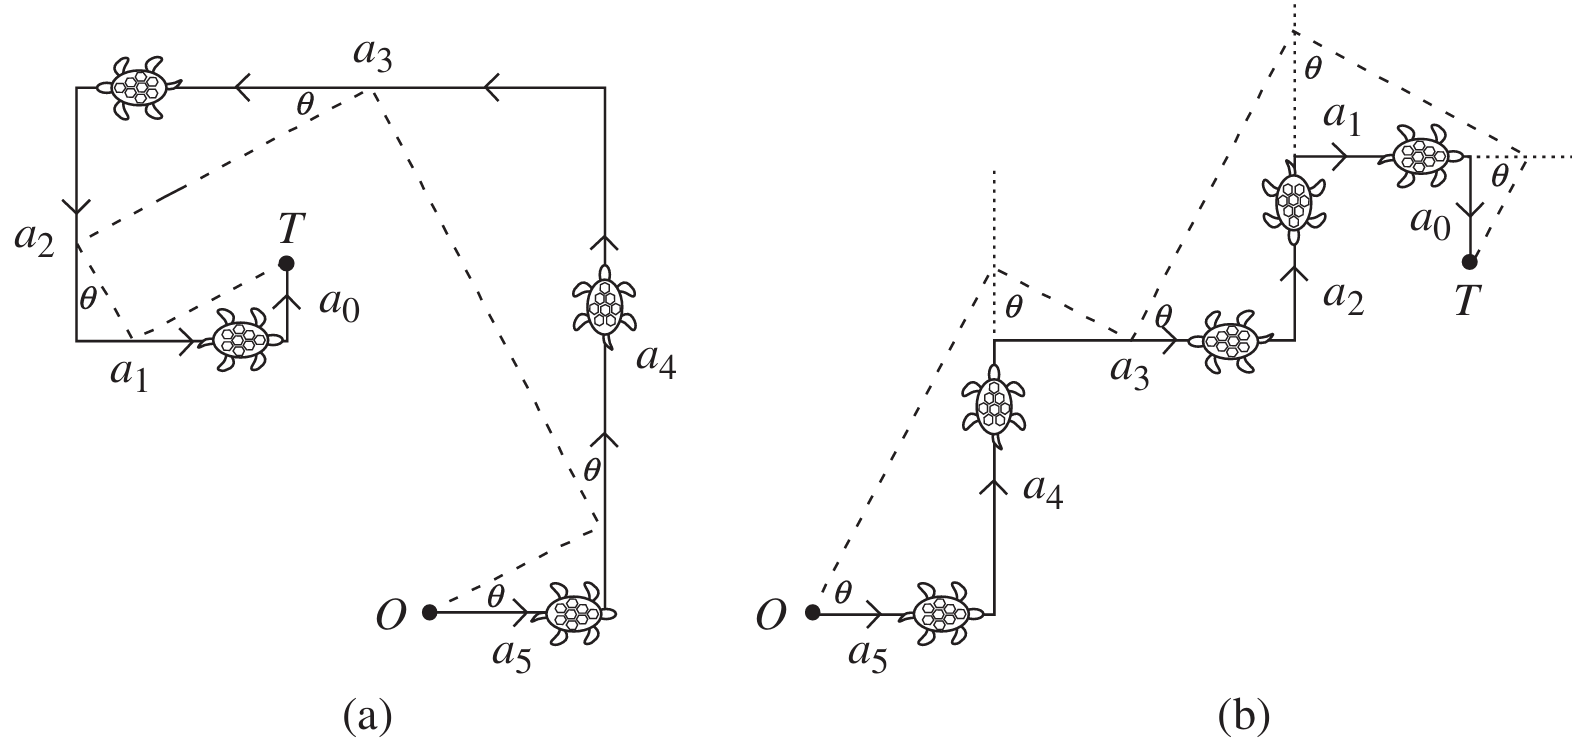
\includegraphics[width=0.9\textwidth]{images/kubična enačba/primera_zelvine_poti.png}
    \caption[Primera želvine poti]{Primera želvine poti za polinoma pete stopnje. Vzeto iz~\cite[str.\ 311]{hull2011}.}
    \label{fig:primera_zelve}
\end{figure}

Sedaj se v izhodišče $O$ postavimo še mi in z laserskim žarkom poskusimo zadeti želvo v točki $T$. Žarek najprej usmerimo daljico $a_{n-1}$, od katere se odbije v daljico $a_{n-2}$, od te v daljico $a_{n-3}$ in tako naprej. (slika~\ref{fig:primera_zelve}). Pri tem upoštevamo troje:
\begin{itemize}
    \item laserski žarek ne upošteva odbojnega zakona in se od daljice vedno odbije pod kotom $90^\circ$, zato so vpadni koti žarka na vse daljice med seboj enaki in prav tako to velja za odbojne kote;
    \item žarek se lahko odbije tudi od nosilke daljice;
    \item vsakič sta možni dve smeri odboja -- na isto stran daljice (oz.\ njene nosilke) ali skoznjo -- izberemo pa tisto, ki nam omogoči, da sploh lahko zadenemo naslednjo daljico.
\end{itemize}
ecimo, da smo zmogli zadeti želvo. Kot, ki ga v točki $O$ oklepata laserski žarek in abscisna os, označimo z $\theta$.

\begin{trditev}
    $x_{\theta} = - \tan \theta$ je ničla polinoma $p(x)$.
\end{trditev}

\begin{dokaz}
    Vzemimo primer, ko so vsi koeficienti polinoma $p(x)$ pozitivni. Želvina pot je v tem primeru sestavljena iz $n+1$ daljic, pot laserskega žarka (ki se vedno odbije od daljice in ne njene nosilke) pa iz $n$ daljic. Slednje so ravno hipotenuze pravokotnih trikotnikov. Za vsako od njih je nasprotna kateta kota $\theta$ del daljice $a_i$, priležno kateto pa označimo z $y_i$ ($ n \geq i \geq 1$). dobimo
    \begin{align*}
        y_n &= \tan \theta \cdot a_n = - x_{\theta} a_n \\
        y_{n-1} &= \tan \theta \cdot (a_{n-1} - y_n) = - x_{\theta} (a_{n-1} + x a_n) = - (a_{n-1} x_{\theta} + a_n x_{\theta}^2)\\
        y_{n-2} &= \tan \theta \cdot (a_{n-2} - y_{n-1}) = - x_{\theta} (a_{n-2} + a_{n-1} x_{\theta} + a_n x_{\theta}^2) = \\
        &= - (a_{n-2} x_{\theta} + a_{n-1} x_{\theta}^2 + a_n x_{\theta}^3) \\
        &\vdots \\
        y_1 &= - (a_1 x_{\theta} + a_2 x_{\theta}^2 + \ldots + a_{n-1} x_{\theta}^{n-1} + a_n x_{\theta}^n).
    \end{align*}
    V zadnji enakosti desno stran premaknimo na levo in upoštevamo $y_1 = a_0$. Dobimo ravno $p(x_{\theta}) = 0$, torej je $x_{\theta} = - \tan \theta$ res ničla tega polinoma.

    \textcolor{red}{Primer negativnih koeficientov:~\cite[str.\ 36]{zore2022}.}

    \textcolor{red}{Primer ničelnih koeficientov: isto kot prej, samo se spusti $y_i$ za tisti $i$, za katerega je $a_i = 0$. (\textcolor{red}{???})}
\end{dokaz}

Če pod nobenim kotom $\theta$ ne moremo zadeti želve, je polinom $p(x)$ brez realnih ničel.

Pojavi se nam vprašanje, kako določiti kot $\theta$. Za polinom tretje stopnje je Belocheva preko svojega pregiba našla zelo preprosto rešitev, ki si jo bomo sedaj pogledali.

\subsubsection*{Belochin kvadrat}

Imejmo dani točki $A$ in $B$ ter premici $r$ in $s$. Z origamijem konstruirajmo kvadrat $WXYZ$, kjer oglišče $X$ leži na premici $r$, njegovo sosednje oglišče $Y$ pa na premici $s$. Velja še, da točka $A$ leži na stranici $WX$ (ali njeni nosilki), točka $B$ pa na stranici $ZY$ (ali njeni nosilki, slika~\ref{fig:beloch_kvadrat}).

\begin{figure}[h]
    \centering
    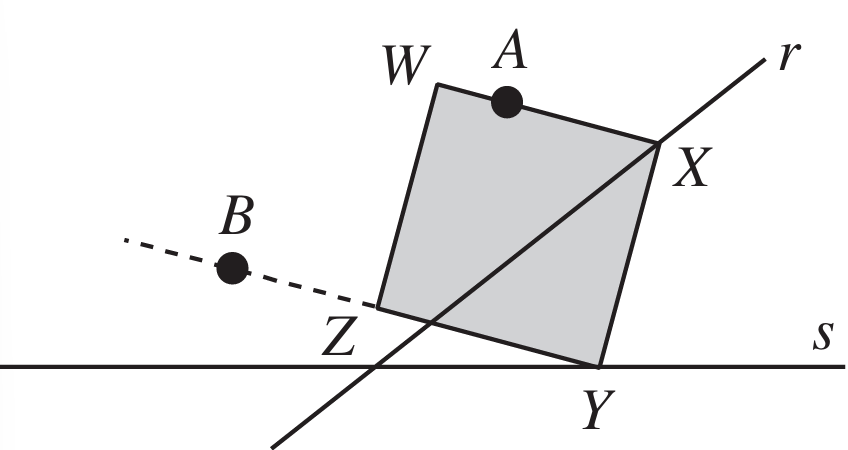
\includegraphics[width=0.4\textwidth]{images/kubična enačba/beloch_kvadrat.png}
    \caption[Belochin kvadrat]{Belochin kvadrat. Vzeto iz~\cite[str.\ 309]{hull2011}.}
    \label{fig:beloch_kvadrat}
\end{figure}

Belocheva je iznašla naslednji postopek, ki nam konstruira ta kvadrat:
\begin{itemize}
    \item Najprej konstruiramo premico $r'$, ki je vzporedna premici $r$ in od nje enako oddaljena kot točka $A$, tako da premica $r$ leži med točko $A$ in premico $r'$. Na enak način premici $s$ konstruiramo njeno vzporednico $s'$ (slika~\ref{fig:beloch_kvadrat_konstrukcija} levo). To konstrukcijo opravimo s prepogibi iz operacije~\ref{op:O5}, zrcaljenja točke čez premico ter ponovne uporabe operacije~\ref{op:O5}. Zaradi preglednosti seveda dopuščamo, da namesto zrcaljenja preprosto prepognemo po premici in s svinčnikom označimo sliko točke.
    \item Nato opravimo Belochin pregib, ki točko $A$ slika v točko $A'$ na premici $r'$, točko $B$ pa v točko $B'$ na premici $s'$ (slika~\ref{fig:beloch_kvadrat_konstrukcija} na sredi).
    \item Naj bo točka $X$ središče daljice $AA'$ in točka $Y$ središče daljice $BB'$. Ker je pregib simetrala teh dveh daljic $AA'$ in $BB'$, sta njuni središči po konstrukciji\footnote{Gledamo lahko dva podobna pravokotna trikotnika s skupnim ogliščem v točki $A$ (oz.\ $B$), enega dvakrat večjega od drugega} ravno presečišči pregiba s premicama $r$ in $s$ (slika~\ref{fig:beloch_kvadrat_konstrukcija} desno).
    \item Daljica $XY$ -- ena izmed stranic kvadrata -- je po konstrukciji pravokotna na daljici $AX$ in $BY$, zato samo še določimo točki $W$ in $Z$ na daljicah ali njunih nosilkah in tako dobimo Belochin kvadrat.
\end{itemize}

\begin{figure}[h]
    \centering
    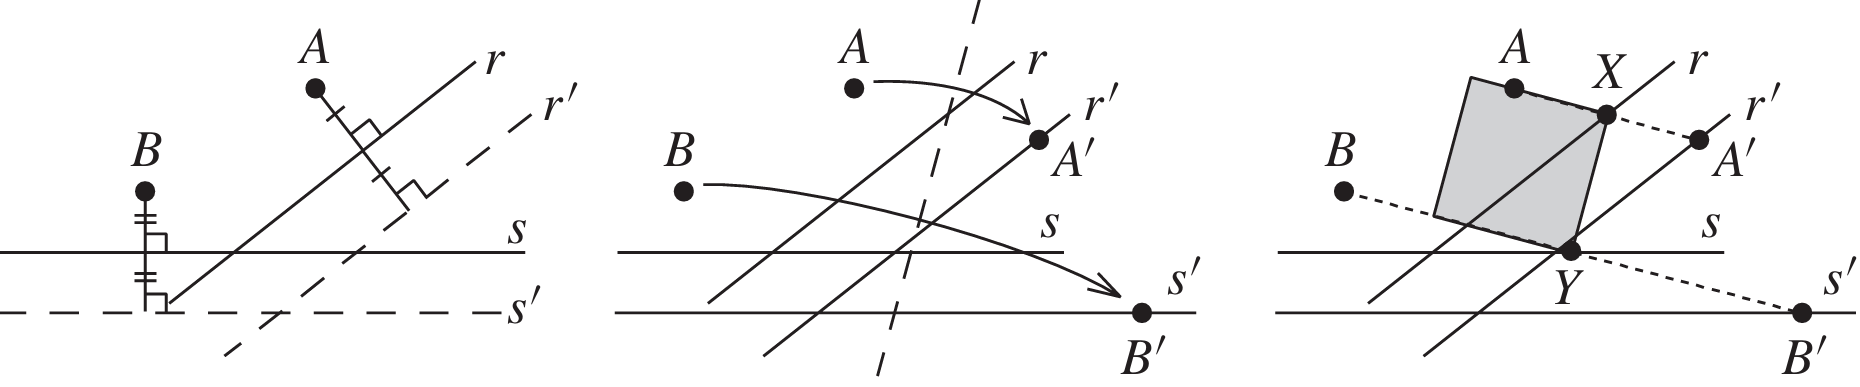
\includegraphics[width=0.95\textwidth]{images/kubična enačba/beloch_kvadrat_konstrukcija.png}
    \caption[Konstrukcija Belochinega kvadrata]{Konstrukcija Belochinega kvadrata z origamijem. Vzeto iz~\cite[str.\ 310]{hull2011}.}
    \label{fig:beloch_kvadrat_konstrukcija}
\end{figure}

\subsubsection*{Konstrukcija $\sqrt[3]{2}$ z Belochinim kvadratom}
\label{podpogl:beloch_kvadrat_koren}

Preden ravno naučeno znanje uporabimo za reševanje kubičnih enačb, si še na hitro poglejmo, kako lahko tudi z Belochinim kvadratom rešimo starogrški problem podvojitve kocke.

Za premico $r$ vzemimo ordinatno os, za premico $s$ pa abscisno os. Določimo še $A = (-1,0)$ in $B = (0, -2)$. Vzporednici sta torej $r': x = 1$ in $s': y = 2$. Belochin pregib seka premico $r$ v točki $X$, premico $s$ pa v točki $Y$ (slika~\ref{fig:beloch_koren}). Z $O$ označimo koordinatno izhodišče in opazimo podobne pravokotne trikotnike $OAX$, $OXY$ in $OYB$. Z upoštevanjem $|AO| = 1 $ in $|OB| = 2$ dobimo sledeča razmerja:
$$ \frac{|OX|}{|AO|} = \frac{|OY|}{|OX|} = \frac{|OB|}{|OY|} \Longrightarrow |OX| = \frac{|OY|}{|OX|} = \frac{2}{|OY|}, $$
iz česar sledi
$$ |OX|^3 = |OX| \cdot \frac{|OY|}{|OX|} \cdot \frac{2}{|OY|} = 2 \Longrightarrow |OX| = \sqrt[3]{2}. $$

\begin{figure}[h]
    \centering
    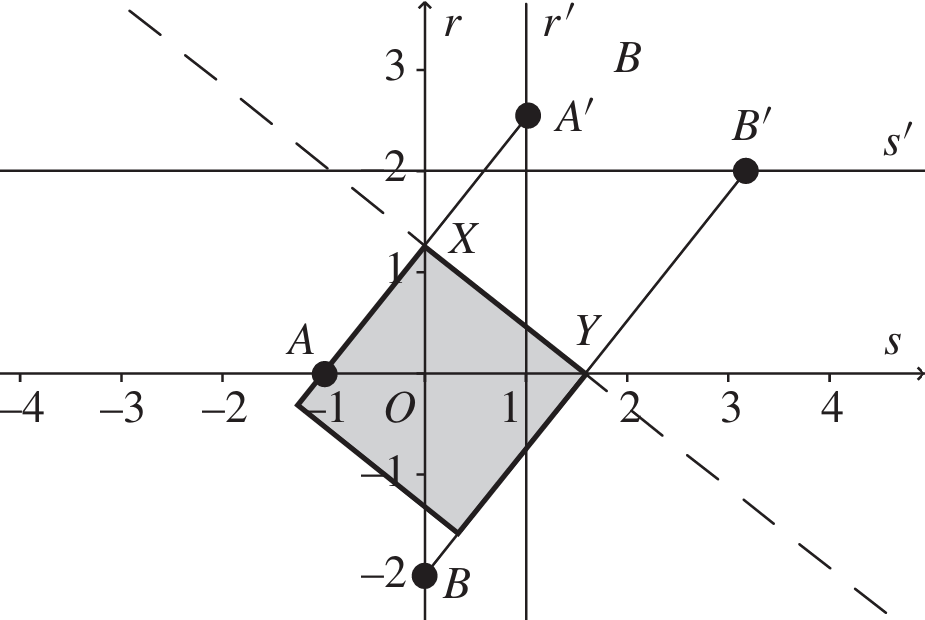
\includegraphics[width=0.5\textwidth]{images/kubična enačba/beloch_koren.png}
    \caption[Konstrukcija kubičnega korena števila dva]{Konstrukcija $\sqrt[3]{2}$ preko Belochinega kvadrata. Vzeto iz~\cite[str.\ 310]{hull2011}.}
    \label{fig:beloch_koren}
\end{figure}

Vidimo lahko, da je to enaka konstrukcija kot jo je 50 let kasneje neodvisno od Belocheve odkril G.\ Martin (razdelek~\ref{podpogl:podvojitev_kocke}), le da je za točko $B$ vzel točko $(0, -k)$ in s tem konstruiral dolžino $\sqrt[3]{k}$ za poljuben origami-konstruktibilen $k$.

\subsubsection*{Združitev Lillove metode in Belochinega kvadrata}

Za poljubno enačbo $a x^3 + b x^2 + c x + d = 0$, kjer $ a \neq 0$, povežimo sedaj Lillovo metodo s konstrukcijo primernega Belochinega kvadrata, ki nam bo natančno določil kot $\theta$. Postopek je sledeč (gl.\ tudi sliko~\ref{fig:beloch_kubicna_resitev}):

\begin{enumerate}
    \item Za točko $A$ vzemimo izhodišče $O$. Začrtamo želvino pot za polinom $p(x) = a x^3 + b x^2 + c x + d$, ki se začne v točki $A$ in konča v točki $B$. V primeru neničelnih koeficientov je pot sestavljena iz štirih stranic, pot laserskega žarka pa iz treh.
    \item Premica $r$ naj bo nosilka daljice $b$ ($r: x = a$), premica $s$ pa nosilka daljice $c$ ($s: y = b$).
    \item Določimo premici $r': x = 2a$ in $s': b + d$ ter opravimo Belochin pregib, ki točko $A$ položi na premico $r'$ in točko $B$ na premico $s'$.
    \item Presečišči pregiba s premicama $r$ in $s$ zaporedoma označimo s točkama $X$ in $Y$.
    \item Zarišemo daljice $AX$, $XY$ in $YB$.
\end{enumerate}

Ker po konstrukciji velja $ AX \perp XY \perp YB $, je to iskana pot laserskega žarka, ki se odbija pod pravim kotom in zadene želvo. Kot $\theta$ je kot, ki ga oklepata daljici $a_3$ in $AX$. Rešitev je torej $x_{\theta} = - \tan \theta$.

\begin{figure}[h]
    \centering
    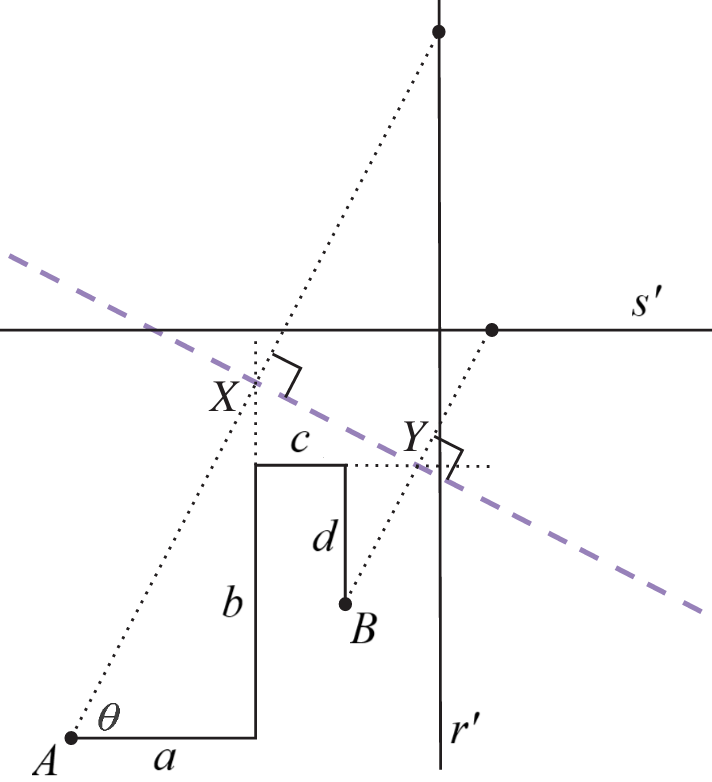
\includegraphics[width=0.4\textwidth]{images/kubična enačba/beloch_kubicna_resitev.png}
    \caption[Lillova metoda z Belochinim kvadratom]{Konstrukcija želvine poti za Lillovo metodo preko Belochinega kvadrata. Vzeto in preurejeno iz~\cite[str.\ 313]{hull2011}.}
    \label{fig:beloch_kubicna_resitev}
\end{figure}

Če ima enačba še dve realni rešitvi, sta možna tudi še dva Belochina pregiba (enačba namreč ne more imeti dveh realnih rešitev, saj kompleksne rešitve nastopajo v konjugiranih parih).

\opomba{V resnici nikoli do sedaj nismo potrebovali konstruirati celega kvadrata; potrebovali smo le stranico $XY$ in dejstvo, da je pregib pravokoten na daljici $AX$ in $BY$.}

\opomba{Enačbe premic $r, s, r'$ in $s'$ so univerzalne in zgornja konstrukcija tako deluje tudi v primeru, ko je kakšen od koeficientov $b, c, d$ ničeln.}

Za konkretne primere uporabe Belochinega postopka za reševanje kubičnih enačb glej~\cite[38--44]{zore2022}.

Kot zanimivost Lavričeva v~\cite[str.\ 10--13]{lavric2013} s postopkom, ki je malo preurejen Belochin postopek, še analitično pokaže, da je ob primerno izbranih točkah $A$ in $B$ ter premicah $r$ in $s$ koeficient tangentnega pregiba rešitev kubične enačbe. Točki in premici izbere tako, da sta točki $X$ in $Y$ ravno presečišči z ordinatnima osema, iz česar lahko takoj razberemo koeficient tangente. V dokazu izpelje enačbi pripadajočih parabol in splošno enačbo njunih tangent ter iz tega dokaže rečeno. To je lahko odlična vaja za dijake, ki si želijo kakšnega izziva.

\subsubsection{Reševanje kvadratne enačbe z Lillovo metodo}
\label{podpodl:kvadr_en_lill}

Lillovo lahko uporabimo tudi za reševanje kvadratne enačbe $a x^2 + b x + c = 0, a \neq 0$. Na enak način v koordinatni sistem zarišemo želvino pot, ki se začne v točki $A$ in konča v točki $B$. Za razliko od prej tu ne uporabimo Belochinega pregiba, temveč pregib iz operacije~\ref{op:O6}. Namesto dveh premic $r$ in $s$ imamo le eno -- naj bo $r$ nosilka daljice $b$. Kot prej -- na razdalji $a$ na drugi strani točke $A$ -- označimo še njeno vzporednico $r'$. Konstruiramo pregib, ki gre skozi točko $B$ in točko $A$ položi na premico $r'$. Njegovo presečišče s premico $r$ nam določi točko $X$, kjer se žarek iz točke $A$ pod pravim kotom odbije v točko $B$. Na sliki~\ref{fig:kv_en_lill} je primer kosntrukcije pri negativnem koeficientu $c$. S tem je kot $\theta$ določen. Premislili smo tudi že, da sta možna največ dva pregiba in da je število pregibov enako številu realnih rešitev enačbe.

\begin{figure}[h]
    \centering
    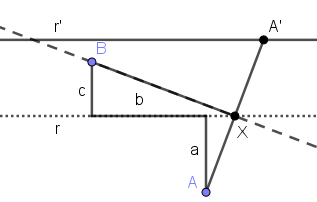
\includegraphics[width=0.5\textwidth]{images/kvadratna_enacba/kvadratna_enacba_lillova_metoda.png}
    \caption[Lillova metoda za kvadratno enačbo]{Reševanje kvadratne enačbe po Lillovi metodi z operacijo~\ref{op:O6} ($c < 0$).}
    \label{fig:kv_en_lill}
\end{figure}

\subsubsection{Hatorijeva konstrukcija}

Japonski matematik Koshiro Hatori navaja postopek, ki je zelo podoben Belochinem postopku, vendar ga je avtor iznašel neodvisno od Belochinega dela. Brez škode za splošnost predpostavi $a = 1$ in za reševanje enačbe $x^3 + bx^2 + cx + d = 0$ sledi naslednjim korakom:
\begin{itemize}
    \item Vkoordinatnem sistemu označimo točki $A = (b, 1)$ in $B = (d, c)$ ter premici $a: y = -1$ in $b: x = -d$.
    \item Opravimo pregib, ki točko $A$ položi na premico $a$ ter točko $B$ na premico $b$ (kar je ravno belochin pregib).
\end{itemize}
Avtor zaključi, da je koeficient opravljenega pregiba rešitev naše enačbe.

Bralec lahko sam premisli, da je to v resnici ravno Belochin postopek, le da se želva na začetku svoje poti ne nahaja v koordinatnem izhodišču in je najprej usmerjena navzdol. Prav tako lahko izrazi koeficient pregiba s kotom ob začetni točki $A$ in res dobi $k = - \tan \theta$. \textcolor{red}{(to si tudi sama preverila in res drži)}. Za geometrijsko razlago preko parabol gl.~\cite{hatori2003}.

\opomba{Seveda bi lahko vzeli katerikoli $a \in \Q$ in vzeli premico $a: y = -a$.}

\subsubsection{Alperinova rešitev}

\textcolor{red}{Tudi on neodvisno od Belocheve, je pa pri njem $a= 1, b = 0$, kar se da nardit z vsako kubično enačbo, pač z uvedno nove spremenljivke al neki, da se kvadratni člen uniči.} (gl.\ Hull 2020 str.\ 43, hull2013 str.\ 78 spodej) - prevedba kubične enačbe na kvadratno al neki tazga.